\chapter{Software Architecture Design}
\label{chap:software-architecture-design}

\section{System Architecture Overview}
\label{section:architecture-overview}
\begin{figure}[h]
    \label{fig:system-diagram}
    \centering
    
\includegraphics[width=1\textwidth]{/diagram/system-diagram.png}
    \caption{System overview diagram}
\end{figure}

This application is developed as a plugin for Unreal Engine. The main workflow begins when a player enters a natural language description at the character creation screen. The plugin constructs a prompt based on the player's input and sends it to an LLM inference service, which operates in one of two modes — online or local — depending on the configuration set by the game developer. The response returned by the LLM is then passed to an adapter layer, which parses the output and converts it into character parameter values. These values are applied to the character's blend shape targets, and the resulting appearance is reflected in a real-time preview shown to the player. System diagram are shown in folowing figure \ref{fig:system-diagram}

\clearpage

\section{Software Design}
\label{section:software-design}
UML Sequence Diagram shown in figure \ref{fig:seq-diagram} showing flow of application in the main use case where user input prompt and generate a character as mention in previous section \ref{section:architecture-overview}
\begin{figure}[h]
    \label{fig:seq-diagram}
    \centering
    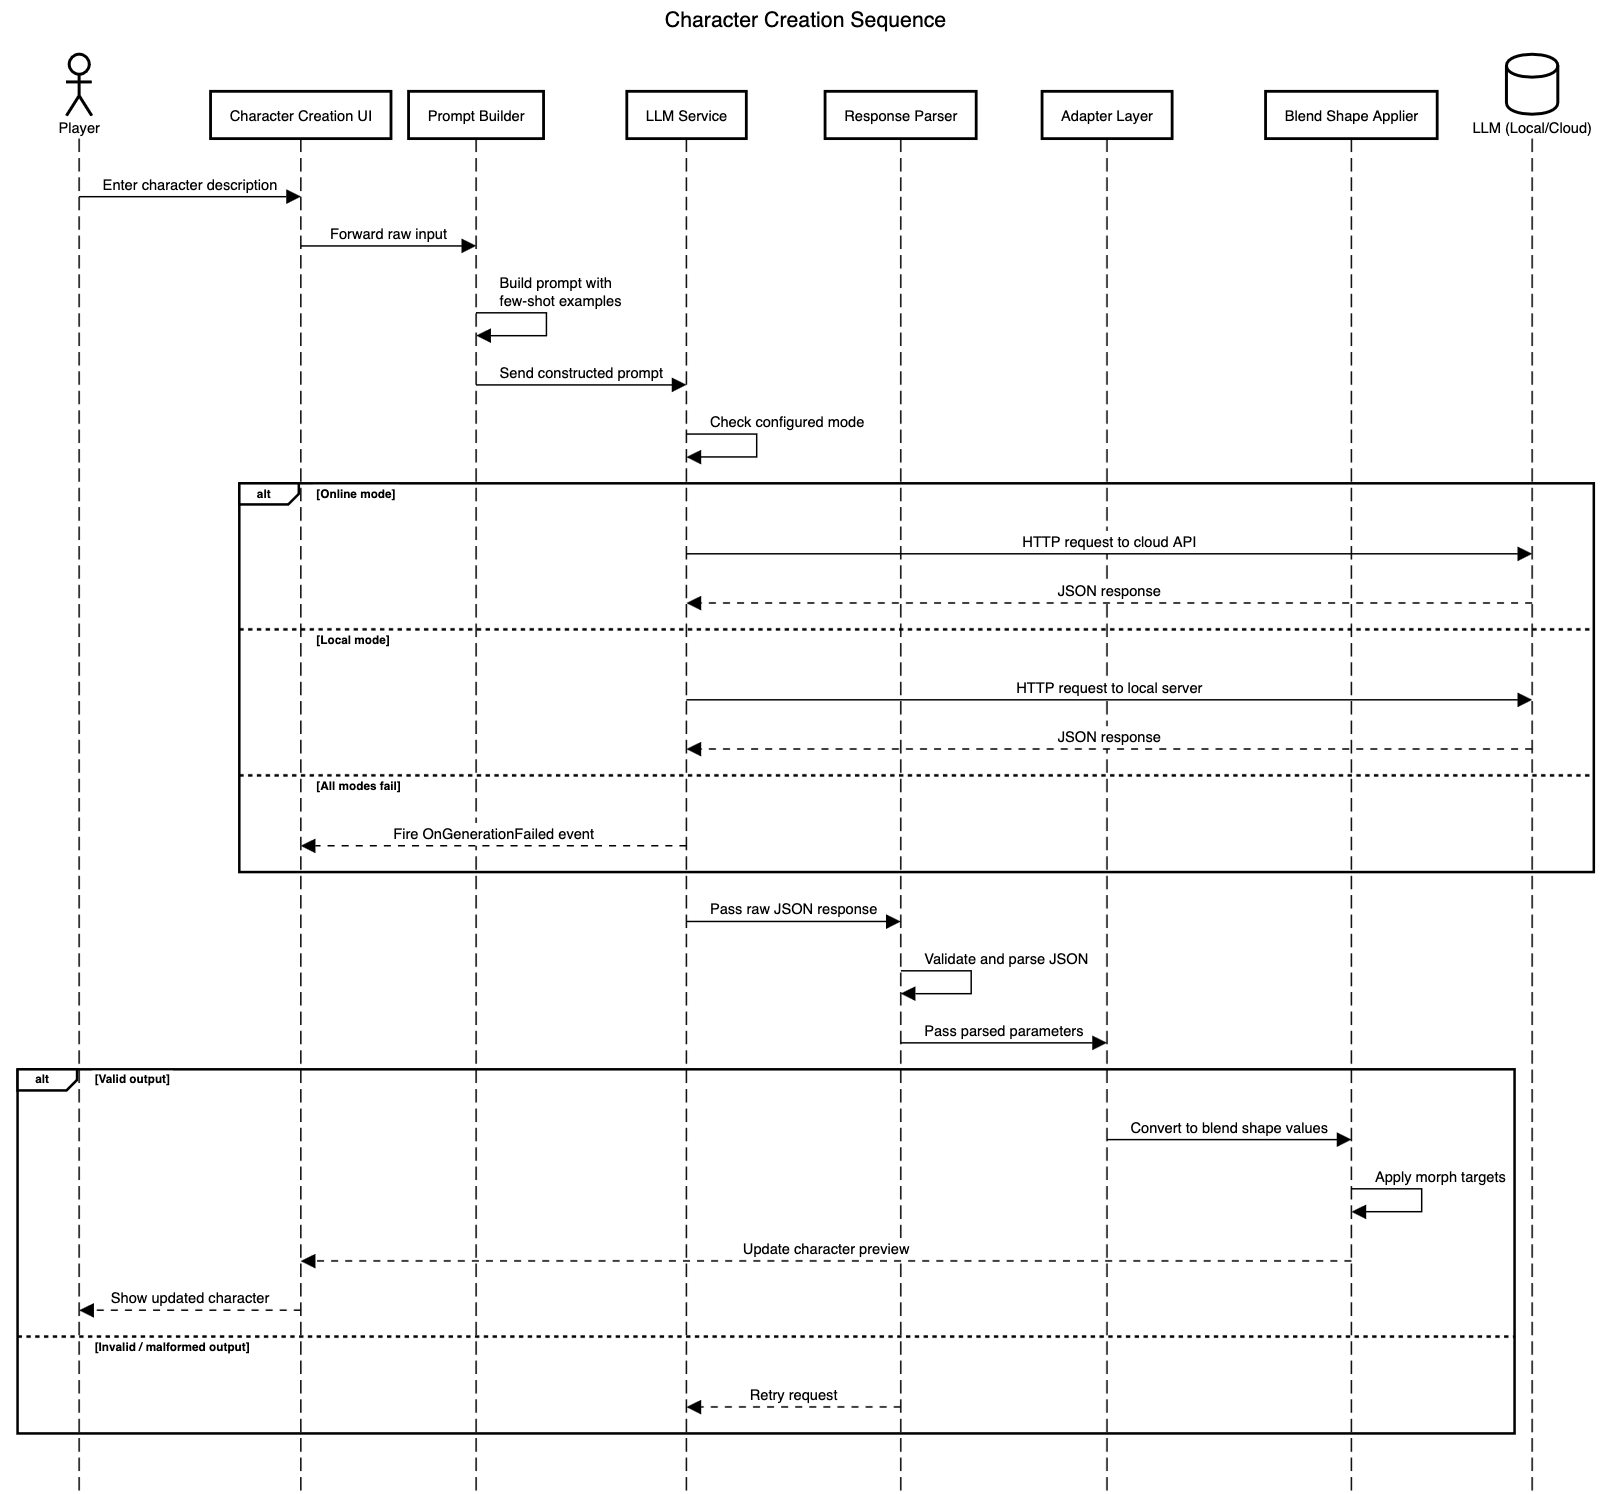
\includegraphics[width=1\textwidth]{assets/diagram/sequence-diagram.png}
    \caption{Sequence diagram of player generating character}
\end{figure}


\section{AI and Data Design}
\label{section:ai-data-design}

\subsection{Data Sources and Collection}
\label{subsection:data-source-col}

This project does not require a dataset for model training or fine-tuning, as the system relies entirely on prompt engineering with pre-trained Large Language Models. All character interpretation capability is derived from the model's existing knowledge rather than task-specific training data.

The primary runtime input to the system is the player's natural language description, entered through the character creation screen. This input is ephemeral — it is constructed into a prompt, sent to the LLM inference service, and discarded after the response is received. No player input is stored or logged by the plugin.

The developer-defined parameter configuration, stored as an Unreal Engine Data Asset, constitutes the only persistent structured data maintained by the system. This includes the list of registered semantic parameters, their expected value ranges, and their mappings to the character mesh's blend shape targets. This configuration is authored once at setup time and does not change at runtime.

For evaluation purposes, a benchmark dataset of approximately 40 to 50 character presets is constructed from an existing character model with known blend shape parameter values. For each preset, multiple natural language prompts are manually authored across varying description styles — including detailed anatomical descriptions, vague impressionistic descriptions, and implied or culturally referenced descriptions such as character archetypes. Each prompt is paired with its corresponding ground truth parameter values extracted directly from the preset. 

\newpage

\subsection{Model Design}


As stated in section \ref{subsection:data-source-col}, this project relies entirely on pre-trained Large Language Models and does not require any model training or fine-tuning. Since the system supports two inference modes — local and cloud — the choice of model varies depending on the mode configured by the developer. Candidate models for each mode are presented below.

The two most critical factors in model selection for this project are the ability to produce reliable structured output in JSON format, and inference performance in terms of response time. For local models, resource consumption must also be considered, as the model runs directly on the player's machine and must operate within reasonable hardware constraints.
\subsubsection*{Cloud Models}

\begin{table}[h]
\centering
\begin{tabular}{|l|c|c|c|}
\hline
\textbf{Feature} & \textbf{GPT-5.4 nano} & \textbf{Gemini 2.5 Flash} & 
\textbf{Claude Haiku 4.5} \\
\hline
Native JSON mode      & \checkmark  & \checkmark  & \checkmark  \\
Instruction following & Good        & Good        & Excellent   \\
Nuanced descriptions  & Good        & Good        & Excellent   \\
Time to first token   & 0.6s        & 0.5s        & 0.7s        \\
Context window        & 400K        & 1M          & 200K        \\
\hline
\end{tabular}
\caption{Cloud LLM model comparison (source: Artificial Analysis \cite{aa_gpt54nano,aa_gemini25flash,aa_claudehaiku45})}
\end{table}

\newpage
\subsubsection*{Local Models}

\begin{table}[h]
\centering
\begin{tabular}{|l|c|c|c|}
\hline
\textbf{Feature} & \textbf{Llama 3.2 3B} & \textbf{Phi-3.5 Mini} & 
\textbf{Gemma 2 2B} \\
\hline
Parameter count            & 3B          & 3.8B        & 2B \\
GBNF constrained decoding  & \checkmark  & \checkmark  & \checkmark \\
Instruction following      & Excellent   & Moderate    & Moderate \\
Minimum RAM                & 4GB         & 4GB         & 2GB \\
\hline
\end{tabular}
\caption{Local LLM model comparison}
\end{table}

\subsection{Evaluation}
The evaluation of this project focuses on two primary aspects: the accuracy of the LLM in producing character parameter values that match the intended character description, and the reliability of the structured output produced by the model.

\textbf{Output Accuracy}
Output accuracy is evaluated using Mean Absolute Error (MAE), which measures the average deviation between the parameter values produced by the LLM and the expected ground truth values extracted from the benchmark dataset. MAE is computed individually for each registered character parameter across all test presets, then averaged into a single overall score representing the model's general accuracy. All character parameter values are normalized to a range of 0 to 1, making MAE scores directly comparable across parameters. The evaluation is further broken down by prompt style — detailed, vague, and implied — to assess how description style affects output accuracy. The following thresholds are used to interpret results:

\begin{table}[h]
\centering
\begin{tabular}{|l|l|}
\hline
\textbf{Overall MAE} & \textbf{Interpretation} \\
\hline
$\leq 0.10$ & Good \\
$0.10 <$ MAE $\leq 0.20$ & Acceptable \\
$> 0.20$ & Poor \\
\hline
\end{tabular}
\caption{MAE threshold interpretation}
\end{table}

\newpage
\textbf{Performance}
Inference performance is measured differently depending on the deployment mode. For cloud inference, Time to First Token (TTFT) is recorded as it reflects the perceived responsiveness from the player's perspective. For local inference, total response time is used instead, since the JSON output is short and generation completes quickly. The target performance thresholds are defined as follows:
\begin{table}[h]
\centering
\begin{tabular}{|l|l|l|}
\hline
\textbf{Mode} & \textbf{Metric} & \textbf{Target} \\
\hline
Local inference  & Total response time & $\leq 8$ seconds \\
Cloud inference  & Time to first token & $\leq 2$ seconds \\
\hline
\end{tabular}
\caption{Performance targets by inference mode}
\end{table}

\textbf{Evaluation Dataset}
All accuracy metrics are computed against a benchmark dataset of approximately 40 to 50 character presets with known ground truth parameter values, as described in Section \ref{subsection:data-source-col} Each preset is paired with multiple prompts across three description styles, giving a total of approximately 120 to 150 individual test cases. Both local and cloud model candidates are evaluated separately against the same dataset to enable direct comparison.
